\documentclass[conference]{IEEEtran}
\usepackage{times}

% numbers option provides compact numerical references in the text. 
\usepackage[numbers]{natbib}
\usepackage{multicol}
\usepackage[bookmarks=true]{hyperref}
\usepackage{amsmath}
\usepackage{amssymb}
\usepackage{graphicx}
\usepackage[table]{xcolor}
\usepackage{multirow}
\usepackage{color}  % For Highlighting

% Editing tools
\newcounter{RamCount}
\newcounter{DavidCount}
\newcounter{BrentCount}
\newcommand{\hilight}[1]{\colorbox{yellow}{#1}}
\newcommand{\David}[1]{\textcolor{red}{\textbf{\theDavidCount}: (#1)} \addtocounter{DavidCount}{1}}
\newcommand{\Ram}[1]{\textcolor{blue}{\textbf{\theRamCount}: (#1)} \addtocounter{RamCount}{1}}
\newcommand{\Brent}[1]{\textcolor{brown}{\textbf{\theBrentCount}: (#1)} \addtocounter{BrentCount}{1}}
\newcommand{\Dan}[1]{\textcolor{magenta}{(#1)}}
\newcommand{\Audrey}[1]{\textcolor{maroon}{(#1)}}

%% Custom macros
\newcommand{\Real}{\mathbb{R}}

\pdfinfo{
   /Author (Daniel Bruder)
   /Title  (Modeling and Control of Soft Robots using the Koopman Operator and Model Predictive Control)
   /CreationDate (D:20101201120000)
   /Subject (Robots)
   /Keywords (Soft Robots; Koopman Operator; Model Predictive Control)
}

\begin{document}

% paper title
\title{Modeling and Control of Soft Robots using the Koopman Operator and Model Predictive Control}

% You will get a Paper-ID when submitting a pdf file to the conference system
\author{Author Names Omitted for Anonymous Review. Paper-ID [add your ID here]}

%\author{\authorblockN{Daniel Bruder}
%\authorblockA{Department of Mechanical Engineering\\
%University of Michigan\\
%Ann Arbor, Michigan 48109\\
%Email: bruderd@umich.edu}
%\and
%\authorblockN{Homer Simpson}
%\authorblockA{Twentieth Century Fox\\
%Springfield, USA\\
%Email: homer@thesimpsons.com}
%\and
%\authorblockN{James Kirk\\ and Montgomery Scott}
%\authorblockA{Starfleet Academy\\
%San Francisco, California 96678-2391\\
%Telephone: (800) 555--1212\\
%Fax: (888) 555--1212}}


% avoiding spaces at the end of the author lines is not a problem with
% conference papers because we don't use \thanks or \IEEEmembership


% for over three affiliations, or if they all won't fit within the width
% of the page, use this alternative format:
% 
%\author{\authorblockN{Michael Shell\authorrefmark{1},
%Homer Simpson\authorrefmark{2},
%James Kirk\authorrefmark{3}, 
%Montgomery Scott\authorrefmark{3} and
%Eldon Tyrell\authorrefmark{4}}
%\authorblockA{\authorrefmark{1}School of Electrical and Computer Engineering\\
%Georgia Institute of Technology,
%Atlanta, Georgia 30332--0250\\ Email: mshell@ece.gatech.edu}
%\authorblockA{\authorrefmark{2}Twentieth Century Fox, Springfield, USA\\
%Email: homer@thesimpsons.com}
%\authorblockA{\authorrefmark{3}Starfleet Academy, San Francisco, California 96678-2391\\
%Telephone: (800) 555--1212, Fax: (888) 555--1212}
%\authorblockA{\authorrefmark{4}Tyrell Inc., 123 Replicant Street, Los Angeles, California 90210--4321}}


\maketitle

\begin{abstract}
%% Why soft robots are useful? (is this needed?)
%% Robots are hard to control
Controlling soft robots with precision is a challenge due in large part to the difficulty of constructing models that are amenable to model-based control design techniques.
% %% Soft robots are well-suited for data-driven methods
% Data-driven modeling methods can be used to address this challenge, since soft robots can safely operate under randomized control inputs and are therefor well suited for  
% are useful since soft robots can be safely  observed operation under randomized control inputs...
%% Koopman operator their offers a solution
Koopman Operator Theory offers a way to construct explicit \emph{linear} dynamical models of soft robots and to control them using established model-based linear control methods.
% by \emph{lifting} state measurements into a higher-dimensional space of real-valued functions and identifying an operator that describes the flow of the system in that space
This method is data-driven, yet unlike other data-driven models such as neural networks, it yields an explicit control-oriented linear model rather than just a ``black-box'' input-output mapping.
%% Summary of contributions
This work describes this Koopman-based system identification method and its application to model predictive controller design.
%% Experiment and results
A model and MPC controller of a pneumatic soft robot arm was constructed via the method, and its performance was evaluated over several trajectory following tasks in the real-world. 
On all of the tasks, the Koopman-based MPC controller outperformed a benchmark MPC controller based on a linear state-space model of the same system.
\end{abstract}

\IEEEpeerreviewmaketitle

%% Insert all content here
\section{Introduction} 
\label{sec:intro}

\David{Sorry Dan, I created a big mess here.  But I was trying to identify your line of reasoning.  Your intro reads well and every sentence is true, but you don't really take your reader by the hand and drag him/her along on the journey towards motivating/justifying your approach.  From what I understand, you would like to say: 1) soft robots are cool but we cannot control them (and hey, animals can do it, so what's the problem?) 2) There are a number of challenges with these continuum systems.  They are infinitely dimensional and nonlinear, which makes even the choice of variables difficult 3) Even if we focus ourselves to input-output control, things remain challenging 4) Some simplified models are okay, but fail when their underlying assumptions don't hold up anymore (as Ram comments, this needs a few examples) 5) data driven models are not well suited for controller design (as Ram comments, this needs elaboration) 6) Koopman stuff and your proposed approach.}
\David{Let me work this backwards:  Before you present your solution (or introduce the Koopman stuff) it would be great if you get the reader to believe what you said on skype the other day "Linear models fail to capture important properties, nonlinear/current data-driven models are very challenging to do control with."  With this in mind, you need two paragraphs preceding this to set up that a) Simple (linear) models fail [including the appropriate citations] and that the nonlinear models who are much better [again, include the appropirate citations] are not as well suited for control. Before that you would need the motivation for soft robots and you need to state what the challenges in controlling them are.}
%% Why soft robots?
%% Body softness has been shown to be useful for robots operating in unstructured/unpredictable environments, or alongside humans, but hard to control.
\Ram{hopefully a picture will appear on the front page?}
Soft-bodied robots \David{"hold the promise to"} can exploit their compliance to adapt to unstructured environments and safely interact with fragile objects \David{extend with other advantages, such as cost and robustness.  Then start new sentence to set the focus of the paper on control.}, but this compliance also makes them challenging to model and control \cite{rus2015design}.
\David{I would turn this around.  First state clearly that current system have not reached the control capabilities of soft systems in nature (setting up your case), then support this claim by the notion that the most successful soft robots are grippers etc. }While the soft robotics community has produced many novel devices such as soft grippers (cite), crawlers (cite), and swimmers (cite), these devices are designed to exploit the flexibility of their bodies to achieve grasping and locomotion and do not exhibit precise control capabilities.
This contrasts with the soft systems found in nature such as octopus arms, elephant trunks, and tongues (cite catapults and catpaws) which simultaneously display unmatched dexterity and adaptability \Ram{I'd try to make the connection between control and dexterity/adaptability more explicit}. \David{In general, I'd be careful with adaptability, because you will not deliver on that.}
The challenge of emulating such versatile behavior with soft robots stems from the inherent difficulty of modeling continuum structures and controlling nonlinear dynamical systems \David{I have not read your results, so I might change some of my comments later.  In general, I'd be a bit worried to set up something that you cannot deliver (full continuum control vs. controlling an output) and instead try to focus your intro on the problem that you can solve.}. 
% can be attributed to two innate characteristics of soft systems: continuum structure, and nonlinear dynamical behavior. 

%% Technical challenges to modeling: continuum structure
% The challenge of modeling and controlling soft robots arises from two innate characteristics: continuum structure, and nonlinear dynamical behavior.
Mathematical models are a convenient tool for predicting behavior and designing controllers for robots, but models are notoriously harder to construct for soft robots than rigid-bodied ones \Ram{citation?}.
Rigid-bodied robots consist of rigid links connected together by discrete joints.
Consequently, there is a natural choice of state variables, i.e. joint deformations, that fully describes the geometry of the system.
Soft robots, in contrast, do not exhibit localized deformation at discrete joints, but instead deform continuously along their bodies.
Therefore, any finite choice of state variables will fall short of fully describing the geometry of a soft robot \Ram{is this obvious? I don't think it is. It is at least worth a citation.} \David{I would also be careful with this claim. 1) I am not sure if this has been sufficiently tried and my guess is that with the right choice of states (some deformation functions maybe), you could get pretty far. 2) By the end of any modelling attempt, you will need to truncate to a finite number of variables.  This includes what you propose.} \David{I think what you'd rather want to say (and how you started the discussion of rigid robots) is that there is no natural choice of what your state is and that this is a very difficult problem.  This would be a more direct lead to your proposed solution.}.
Luckily, most tasks only require the control of a discrete set of output parameters (e.g. only the location of a robot's end effector may be relevant for a pick-and-place task). \David{I am a bit lost in what you set up here.  It first seems a bit like you try to set up a case of why input output control is inferior yet then focus on that.}  \David{To be a bit more constructive: I would almost suggest to say something along the lines of "even for simple input-output models this is a very hard problem"}
Input-output models, rather than complete state-space models \Ram{that describe the configuration of the entire soft robot}, are sufficient in such cases, which is why
simplified models, notably the piecewise constant curvature (\cite{webster2010design}), pseudo-rigid-body (cite), and quasi-static models \cite{bruder2018iros} (cite others), have been developed to capture the most salient features of soft systems.
These models have been found to be sufficiently accurate for some objectives (cite), but they still fall short in scenarios where the underlying model assumptions break down \Ram{can you give an example.} \David{I feel this is what your intro should lead to.  That these simplified models are not sufficient.} \David{I feel that other issues, such as nonlinearities, unclear mass distribution, non-holonomic behavior,... could also be addressed as challenges that you are able to solve.}.
Another approach has been to utilize data-driven methods such as neural networks \cite{gillespie2018learning} to construct input-output models.
While such ``black-box'' models have been shown to predict behavior well, they offer little insight when it comes to the design of controllers \Ram{can you be more explicit here?} \David{I liked how you described this on the phone.  "Linear models don't capture everything, nonlinear models are not good for control."  I think your last paragraph before the Koopman stuff needs to end with this line.}.


%% Technical challenge to control: Nonlinear dynamical behavior (think about this more and fix it)
Any model that adequately captures the input-output behavior of a soft robot almost certainly contains nonlinearities \David{I know that you want this here to set up your approach, but I feel that you need to introduce nonlinearities sooner as a challenge }, which presents a control challenge.
Linear dynamical systems obey the \emph{superposition principle} (cite), which has enabled the development of powerful tools that render the task of controlling linear systems almost trivial.
Unfortunately, the superposition principle does not hold for nonlinear dynamical systems and consequently there is no universal approach to controlling them.
Due to the continual increases in computational power and affordability, numerical control techniques have become a popular approach.
However, these methods require solving nonlinear optimization problems which may not be convex.
Thus numerical solvers may converge to suboptimal local extrema rather than optimal values.
% they are also slow...

% While this problem is not limited to soft robots (few mechanical systems exhibit completely linear dynamic behavior), soft robots are not as amenable to approximate linear descriptions as many other systems.

% linear models are especially unfit to describe them.
% rigid-bodied robots have have a linear mapping from joint velocities to end effector velocities through a state-dependent Jacobian matrix
% and a well-developed body of literature dedicated to control methods for robots of this type (see \citet{spong2008robot} for a survey).
% No such body of literature yet exists for soft robots
% Some effort has been made to apply Jacobians to soft robotic systems, but such efforts are limited to quasi-static (cite my RAL paper) cases.
% The nonlinearities presented by soft robots are harder to deal with for this reason.
% Nonlinear control methodologies do not have the same guarantees as linear control (can probably find citation for this)

%% FIGURE: Overview of the different system representations and control approaches
\begin{figure}
    \centering
    \includegraphics[width=\linewidth]{figures/overview_v5_ph.png}
    \caption{Caption}
    \label{fig:overview}
\end{figure}


%% Koopman approach exists and can help here, it just needs some tweaks to work well for a real system
Koopman Operator Theory offers an approach that can overcome the challenges of modeling and controlling nonlinear continuum systems.
Laid out in \citet{mauroy2016linear} and \citet{korda2018linear}, the approach leverages the linear structure of the Koopman operator to construct linear models for nonlinear controlled dynamical systems from input-output data, and control them using established linear control methods (such as model predictive control) \Ram{1. prolly want to cite our paper. 2. only the mezic paper does control. 3. probably want to cite the todd murphey paper.}.
In theory, this approach involves \emph{lifting} the state-space to an infinite-dimensional space of scalar functions (referred to as observables), where the flow of such observables along trajectories of the nonlinear dynamical system is described by the \emph{linear} Koopman operator.
In practice, however, it is not feasible to compute an infinite-dimensional operator, so a modified version of the Extended Dynamic Mode Decompostion (EDMD) is employed to compute a finite-dimensional projection of the Koopman operator onto a finite-dimensional subspace of all observables (scalar functions).
This approximation of the Koopman operator describes the evolution of the values of the output variables themselves, provided that they lie within the finite subspace of observables upon which the operator is projected.
Hence, this approach makes it possible to control the output of a nonlinear dynamical system using linear controllers designed for its linear Koopman representation \Ram{probably want to describe the shortcomings of this approach first?}.

%% Why this approach is uniquely well suited for soft robots: 
The Koopman approach to modeling and control is well suited for soft robots for several reasons.
Soft robots pose less of a physical threat to themselves or their surroundings when subjected to random control inputs than many conventional rigid bodied robots. 
This makes it possible to safely collect input-output data over a wide range of operating conditions, and to do so in an automated fashion. 
Furthermore, since the Koopman procedure is entirely data-driven, it inherently captures input-output behavior and avoids the ambiguity involved in choosing a discrete set of states for a continuum structure that has infinite degrees of freedom.
Soft robots are also nonlinear dynamical systems, but this approach generates a linear system representation.
As will be shown later, this linear representation can be used to construct a numerical controller which computes control inputs by solving a convex optimization problem at each time step.

%% Our contribution: Modifications/additions needed to get this to reliably work for a real system
\Ram{probably worth listing out all your contributions.}
In this work, we modify the Koopman system identification procedure of \citet{mauroy2016linear} and \citet{korda2018linear} to increase its efficacy when applied to real mechanical systems.
Specifically, we introduce an L1 penalty term into the least-squares optimization problem used to solve for the approximate Koopman operator.
This penalty term makes the result more robust to outliers in the training data, and promotes sparseness of the matrix representation of the operator.
Both of these are desirable features when working with real systems, which suffer from noise and computational limitations.

\Dan{Add comment about how real systems like ours have noise and need regularization (LASSO) to combat that in the model fit... (figure out best place to put it).}



%% Outline
The rest of this paper is organized as follows:
In Section \ref{sec:sysid} we formally introduce the Koopman operator and describe the procedure for constructing linear models of nonlinear systems. 
In Section \ref{sec:mpc} we describe how the Koopman model can be used to construct a linear model predictive controller for a nonlinear dynamical system.
In Section \ref{sec:methods} we describe the soft robot used in our experiments and the various other controllers used for comparison.
In Section \ref{sec:results} we summarize the performance of each controller at given trajectory following tasks.
In Section \ref{sec:conclusion} concluding remarks and perspectives are provided.





% %% Solution: Data-driven/linear representation, description of koopman approach
% In this paper, we present a novel method for the modeling and control of soft robots based on Koopman Operator Theory.
% This method addresses the challenges of modeling and control by offering a way to build a \emph{linear} model from data that still captures the \emph{nonlinear} input-output behavior of a soft robot.
% This approach is based on the system identification method originally presented in \citet{mauroy2017koopman} and the control approach laid out in \citet{korda2018linear}.
\section{Linear System Identification}
\label{sec:sysid}

%% Overview of this section
Any finite-dimensional, Lipschitz continuous nonlinear dynamical system has an equivalent infinite-dimensional linear representation that acts on the space of all real-valued functions on the system's state \cite[Definition 3.3.1]{lasota2013chaos}.
This linear representation, which is called the Koopman operator, describes the flow of functions along trajectories of the system.
% The dual of the Koopman operator, the Perron-Frobenius operator, describes the dynamics of the system...
While it is not possible to numerically represent the infinite-dimensional Koopman operator, it is possible to construct its projection onto a finite-dimensional subspace using a matrix.
% Our goal is to construct models in this subspace in the form of a controlled linear dynamical system
% \begin{align}
%     \psi_{k+1} &= A \psi_{k} + B u_{k} \\
%     y_{k} &= C \psi_{k}
% \end{align}
% where $z$ is ... , $u$ is the input, and $y$ is the output of the system.
This section shows that for a given choice of basis functions, a \emph{lifted} linear dynamical system model can be extracted directly from the matrix approximation of the Koopman operator.
% As desired, system representations of this form lend themselves to linear control methods.
The remainder of this sections outlines the approach for constructing the Koopman operator approximation and the linear system representation from data.
Section \ref{sec:mpc} illustrates how this model can be incorporated into a model predictive control algorithm.

%% Overview of the Koopman operator and how it represents dynamical systems
\subsection{Koopman Representation of a Dynamical System}

%% System representation in state space
Consider a dynamical system
\begin{align}
    \dot{x}(t) &= F (x(t))
    \label{eq:nlsys}
\end{align}
where $x(t) \in X \subset \Real^n$ is the state of the system at time $t \geq 0$, $X$ is a compact subset, and ${F}$ is a continuously differentiable function.
Denote by $\phi(t,x_0)$ the solution to \eqref{eq:nlsys} at time $t$ when beginning with the initial condition $x_0$ at time $0$.
For simplicity, we denote this map, which is referred to as the \emph{flow map}, by $\phi_t (x_0)$ instead of $\phi (t, x_0)$.

%% System representation in the space of observables
The system can be lifted to an infinite dimensional function space $\mathcal{F}$ composed of all square integrable real-valued functions with compact domain $X \subset \Real^n$.
Elements of $\mathcal{F}$ are called \emph{observables}.
In $\mathcal{F}$, the flow of the system is characterized by the set %semigroup 
of Koopman operators 
$U_t : \mathcal{F} \to \mathcal{F}$, for each $t \geq 0$,
which describes the evolution of the observables ${f \in \mathcal{F}}$ along the trajectories of the system according to the following definition:
\begin{align}
    U_t f = f \circ \phi_t,      
    % && \forall f \in \F, t \geq 0
    \label{eq:koopman}
\end{align}
where $\circ$ indicates function composition.
As desired, $U_t$ is a linear operator even if the system \eqref{eq:nlsys} is nonlinear, since for $f_1, f_2 \in \mathcal{F}$ and $\lambda_1, \lambda_2 \in \Real$
\begin{align}
    \begin{split}
    U_t (\lambda_1 f_1 + \lambda_2 f_2) &= \lambda_1 f_1 \circ \phi_t + \lambda_2 f_2 \circ \phi_t \\
    &= \lambda_1 U_t f_1 + \lambda_2 U_t f_2.
    \end{split}
\end{align}
Thus the Koopman operator provides a linear representation of the flow of a nonlinear system in the infinite-dimensional space of observables (see Fig. \ref{fig:overview}) \cite{budivsic2012applied}.
Contrast this representation with the one generated by the (nonlinear) flow map that for each $t \geq 0$ describes how the initial condition evolves according to the dynamics of the system.
In particular if one wants to understand the evolution of an initial condition $x_0$ at time $t$ according to \eqref{eq:nlsys}, then one could solve the nonlinear differential equation to generate the flow map. 
On the other hand, one could apply $U_t$ (a linear operator) to the indicator function centered at $x_0$ (i.e. the function that is $1$ at $x_0$ and zero everywhere else) to generate an indicator function centered at the point $\phi_t(x_0)$.
% \Ram{you need to say something more explicit here. While $\phi$ describes how an initial condition flows according to the ODE, the Koopman operator describes how a function evolves according to the ODE. Notice that one can go back and forth between the representations...}.


%% Koopman-based system identification (consult ICRA paper)
\subsection{Identification of Koopman Operator}
\label{sec:koopid}

Since the Koopman operator is an infinite-dimensional object, it cannot be represented by a finite-dimensional matrix. 
Therefore, we settle for the projection of the Koopman operator onto a finite-dimensional subspace.
Using a modified version of the Extended Dynamic Mode Decomposition (EDMD) algorithm \cite{williams2015data} originally presented in \cite{mauroy2016linear,mauroy2017koopman}, we identify a finite-dimensional approximation of the Koopman operator via linear regression applied to the observed data.

Define ${\bar{\mathcal{F}} \subset \mathcal{F}}$ to be the subspace of $\mathcal{F}$ spanned by ${N>n}$ linearly independent basis functions 
${ \{ \psi_i : \Real^n \to \Real \}_{i=1}^N}$.
We denote the image of $\psi_k$ as $ \mathcal{R}_k$ which is equal to ${ \{ w \in \Real | \exists x \in \Real^n \text{ such that } \psi_i(x) = w  \} }$.
For convenience, we assume that the first $n$ basis functions are defined as
\begin{align}
    &\psi_i(x) = x_i
    \label{eq:xinpsi}
\end{align}
where $x_i$ denotes the $i^{\text{th}}$ element of $x$.
Any observable $\bar{f} \in \bar{\mathcal{F}}$ can be expressed as a linear combination of elements of these basis functions
\begin{align}
    \bar{f} &= \theta_1 \psi_1 + \cdots + \theta_N \psi_N
    \label{eq:fexpanded}
\end{align}
where each $\theta_i \in \Real$.
To aid in presentation, we introduce the vector of coefficients ${\theta = [ \theta_1 \,  \cdots \, \theta_N ]^\top}$ and the \emph{lifting function} ${\psi : \Real^n \to \Real^N}$ defined as:
\begin{align}
    % \psi(x) &:= \begin{bmatrix} \psi_1 (x) & \cdots & \psi_N (x) \end{bmatrix}^\top.
    \psi(x) &:= \begin{bmatrix} x_i & \cdots & x_n & \psi_{n+1} (x) & \cdots & \psi_N (x) \end{bmatrix}^\top.
    \label{eq:lift}
\end{align}
We denote the image of $\psi$ as $\mathcal{M} = \mathcal{R}_1 \times \cdots \times \mathcal{R}_N \subset \Real^N$.
By \eqref{eq:fexpanded} and \eqref{eq:lift}, $\bar{f}$ evaluated at a point $x$ in the state space is given by
% Note that $\bar{\theta}$ provides a vector representation for ${ \bar{f} \in \bar{\mathcal{F}} }$, and $\bar{f}$ evaluated at a point $x$ is given by
% Then, $\bar{f} \in \bar{\mathcal{F}}$ can be expressed concisely as
\begin{align}
    \bar{f}(x) &= \theta^\top \psi (x)
    \label{eq:fvec}
\end{align}
We therefore refer to $\psi(x)$ as the \emph{lifted state}, and $\theta$ as the \emph{vector representation} of $\bar{f}$.

Given this vector representation for observables, a linear operator $L : \bar{\mathcal{F}} \to \bar{\mathcal{F}}$ can be represented as an ${N \times N}$ matrix. 
We denote by $\bar{U}_t \in \Real^{N \times N}$ the approximation of the Koopman operator in $\bar{\mathcal{F}}$, which operates on observables via matrix multiplication:
\begin{align}
    \bar{U}_t \theta = \theta'
\end{align}
where $\theta , \theta'$ are each vector representations of observables in $\bar{\mathcal{F}}$.
%% Pulled straight from ICRA paper below this line
Our goal is to find a $\bar{U}_t$ that describes the action of the infinite dimensional Koopman operator $U_t$ as accurately as possible in the $L^2$-norm sense on the finite dimensional subspace $\bar{\mathcal{F}}$ of all observables.

To perfectly mimic the action of $U_t$ on an observable ${f \in \bar{\mathcal{F}} \subset \mathcal{F}}$, according to \eqref{eq:koopman} the following should be true for all  $x \in X$
\begin{align}
    \bar{U}_t \bar{f}(x) &= \bar{f} \circ \phi_t(x) \\
    ( \bar{U}_t {\theta} )^\top {\psi}(x) &=
    {\theta}^\top {\psi} \circ \phi_t(x) \\
    \bar{U}_t^\top \psi(x) &= {\psi} \circ \phi_t(x),
    \label{eq:UbarEq}
\end{align}
where the second equation follows by substituting \eqref{eq:fexpanded} and the last equation follows by cancelling $\theta^\top$.
Since this is a linear equation, it follows that for a given ${x \in X}$, solving \eqref{eq:UbarEq} for $\bar{U}_t$ yields the best approximation of $U_t$ on $\bar{\mathcal{F}}$ in the $L^2$-norm sense \cite{penrose1956best}:
\begin{align}
    \bar{U}_t = \left( {\psi}^\top(x) \right)^\dagger ( {\psi} \circ \phi_t(x) )^\top
    \label{eq:Uapprox}
\end{align}
where superscript $\dagger$ denotes the least-squares pseudoinverse.

%% How this is done on our system
To approximate the Koopman operator from a set of experimental data, we take $K$ discrete state measurements in the form of so-called ``snapshot pairs'' $(a[k] , b[k])$ for each $k \in \{1,\ldots,K\}$ where
% with sampling period $T_s$. We separate the data into a set of $K$ so-called ``snapshot pairs'' of the form ${ \{ a_k , b_k \} \in \Real^{n \times 2} }$ where
\begin{align}
    a[k] &= x[k] \\
    b[k] &= \phi_{T_s} (x[k]) + \sigma[k],
    \label{eq:ab}
\end{align}
where $\sigma_k$ denotes measurement noise, $T_s$ is the sampling period which is assumed to be identical for all snapshot pairs, and $x[k]$ denotes the measured state corresponding to the $k^\text{th}$ measurement.
% \Ram{is this where we mention that these measurements do not have to correspond to the state of the system but rather the things we can observe?}
Note that consecutive snapshot pairs do not have to be generated by consecutive state measurements. 
% For our basis of $\bar{\mathcal{F}}$, we choose the basis of monomials of $x$ with total degree less than or equal to $w$, which implies ${N=(n+m+w)!/\left((n+m)!w!\right)}$ \cite[Section III]{mauroy2016linear}. 
We then lift all of the snapshot pairs according to \eqref{eq:lift} and compile them into the following ${K \times N}$ matrices:
\begin{align}
    &\Psi_a := \begin{bmatrix} {\psi}(a[1])^\top \\ \vdots \\  {\psi}(a[K])^\top \end{bmatrix}
    &&\Psi_b := \begin{bmatrix} {\psi}(b[1])^\top \\ \vdots \\  {\psi}(b[K])^\top \end{bmatrix}
    \label{eq:Psi}
\end{align}
$\bar{U}_{T_s}$ is chosen so that it yields the least-squares best fit to all of the observed data, which, following from \eqref{eq:Uapprox}, is given by 
\begin{align}
    \bar{U}_{T_s} &:= \Psi_a^\dagger \Psi_b.
\end{align}

%% Incorporating Delays
Sometimes a more accurate model can be attained by incorporating delays into the set of snapshot pairs. 
To incorporate these delays, we define the snapshot pairs as
\begin{align}
    a[k] &= \begin{bmatrix} x[k]^\top, & x[k-1]^\top & \ldots, & x[k-d]^\top \end{bmatrix}^\top \label{eq:snapd1} \\
    b[k] &= \begin{bmatrix} \left( \phi_{T_s} (x[k]) + \sigma_k \right)^\top & x[k]^\top & \ldots & x[k-d+1]^\top \end{bmatrix}^\top \label{eq:snapd2}
\end{align}
where $d$ is the number of delays.
We then modify the domain of the lifting function such that $\psi : \Real^{n+nd} \to \Real^{N}$ to accommodate the larger dimension of the snapshot pairs.
Once these snapshot pairs have been assembled, the model identification procedure is identical to the case without delays.
% without input delays or $\Real^{n+nd} \times \Real^{md}$ with input delays.

%% Koopman representation of controlled dynamical system
\subsection{Building Linear System from Koopman Operator}
%Brent: Building a Linear Model from the Koopman Operator
% I don't get the lack of articles in your section heading. 

For dynamical systems with inputs, we are interested in using the Koopman operator to construct discrete linear models of the following form
\begin{equation}
\begin{aligned}
    z[j+1] &= A z[j] + B u[j] \\
    x[j] &= C z[j]
    \label{eq:linSys}
\end{aligned}
\end{equation}
for each $j \in \mathbb{N}$, where $x[0]$ is the initial condition in state space, $z[0] = \psi(x[0])$, $u[j] \in \Real^m$ is the input at the $j^{\text{th}}$ step, and $C$ acts as a projection operator from the lifted space onto the state-space.
Specifically, we desire a representation in which (non-lifted) inputs appear \emph{linearly}, because models of this form are amenable to real-time, convex optimization techniques for feedback control design as we describe in Section \ref{sec:mpc}.

We construct a model of this form by first applying the system identification method of Section \ref{sec:koopid} to the following modified snapshot pairs
% \begin{align}
%     \alpha_k &= \begin{bmatrix} \psi(a_k)^\top & u_k^\top \end{bmatrix} \\
%     \beta_k &= \begin{bmatrix} \psi(b_k)^\top & u_k^\top \end{bmatrix} 
% \end{align}
\begin{align}
    &\alpha[k] = \begin{bmatrix} \psi(a[k]) \\ u[k] \end{bmatrix} 
    &&\beta[k] = \begin{bmatrix} \psi(b[k]) \\ u[k] \end{bmatrix}
    \label{eq:alpha}
\end{align}
for each $k \in \{1,\ldots,K\}$. 
The input $u[k]$ in snapshot $k$ is not lifted to ensure that it appears linearly in the resulting model.
With these pairs, we define the following ${K \times (N + m)}$ matrices:
\begin{align}
    &\Gamma_\alpha = \begin{bmatrix} \alpha[1]^\top \\ \vdots \\  \alpha[K]^\top \end{bmatrix}
    &&\Gamma_\beta = \begin{bmatrix} \beta[1]^\top \\ \vdots \\  \beta[K]^\top \end{bmatrix}
    \label{eq:Gamma}
\end{align}
and solve for the corresponding Koopman operator according to \eqref{eq:Uapprox}
\begin{align}
    \bar{U}_{T_s} &:= \Gamma_{\alpha}^\dagger \Gamma_\beta.
    \label{eq:koopGamma}
\end{align}
Note that by \eqref{eq:UbarEq} and \eqref{eq:koopGamma} the transpose of this Koopman matrix is the best approximation of a transition matrix between the elements of snapshot pairs in the $L^2$-norm sense \
\begin{align}
    \bar{U}_{T_s}^\top 
    \begin{bmatrix} \psi(a[k]) \\ u[k] \end{bmatrix} &\approx
    \begin{bmatrix} \psi(b[k]) \\ u[k] \end{bmatrix},
\end{align}
and we desire the best $A,B$ matrices such that
\begin{align}
    A \psi(a[k]) + B u[k] &\approx \psi(b[k])
    \label{eq:linSys_psi}
\end{align}
Therefore, the best $A$ and $B$ matrices of \eqref{eq:linSys} are embedded in $\bar{U}_{T_s}^\top$ and can be isolated by partitioning it as follows:
\begin{align}
    \bar{U}_{T_s}^\top &= 
    \begin{bmatrix} 
        A_{N \times N} &
        B_{N \times m} \\
        O_{m \times N} &
        I_{m \times m}
    \end{bmatrix}
    \label{eq:AB}
\end{align}
where $I$ denotes an identity matrix, $O$ denotes a zero matrix, and the subscripts denote the dimensions of each matrix.
The $C$ matrix is defined
\begin{align}
    C &= \begin{bmatrix} I_{n \times n} & O_{n \times (N-n)} \end{bmatrix}
    \label{eq:C}
\end{align}
since by \eqref{eq:xinpsi}, ${x = [ \psi_1(x) , \dots , \psi_n(x) ]}$.
Note we can also incorporate input delays into the model by appending them to the snapshot pairs as we did in \eqref{eq:snapd1} and \eqref{eq:snapd2}.


% \begin{align}
%     z_{k+1} &= A z_k + B u_k
%     \label{eq:linSys}
% \end{align}

% \begin{align}
%     \begin{bmatrix} \psi(b_k) \\ u_k \end{bmatrix} &=
%     \begin{bmatrix} A_{N \times N} & B_{N \times m} \\ O_{m \times N} & I_{m \times m} \end{bmatrix} 
%     \begin{bmatrix} \psi(a_k) \\ u_k \end{bmatrix}
% \end{align}


%% Why should we use lasso instead of the least-squares solution
\subsection{Practical Considerations: Overfitting and Sparsity} \label{subsec:sparsity}


%% FIGURE: Lifting and Projecting
\begin{figure}
    \centering
    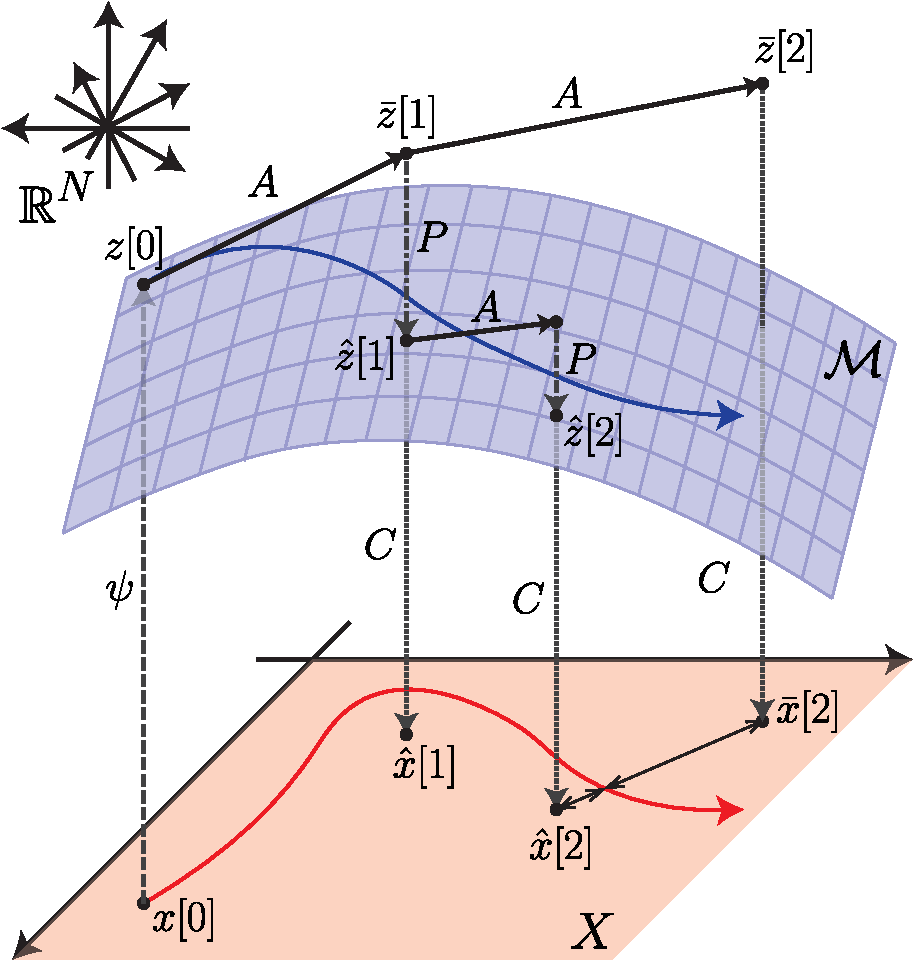
\includegraphics[width=0.8\linewidth]{figures/liftingManifold_v17.pdf}
    \caption{An illustration of the effect of deviating from the image of the lifted functions ${\cal M}$ and how it can be remedied by defining a projection operation as described in Section \ref{subsec:sparsity}. 
    The evolution of the finite dimensional system in the state space $X$ from $x_0$ is depicted as a red curve. 
    The lifted version of this evolution is depicted as the blue curve which is contained in $\cal{M}$.
    The discrete time system representation in the higher-dimensional space created by iteratively applying the state matrix $A$ to $z[j]$ may generate a solution that is outside of ${\cal M}$.
    Though one can still apply $C$ to $\bar{z}$ to project it back to $X$, this may result in poor performance.
    Instead, by projecting $\bar{z}[j]$ onto the manifold at each discrete time step to define a new lifted state $\hat{z}[j]$, the deviation from $\cal{M}$ is reduced, which improves overall predictive performance. }
    \label{fig:manifold}
    \vspace*{-0.5cm}
\end{figure}

%% Need a way to deal with outliers
A pitfall of data-driven modeling approaches is the tendency to overfit.
While least-squares regression yields a solution that minimizes the total $L^2$ error with respect to the training data, this solution can be particularly susceptible to outliers and noise \cite{rousseeuw2005robust}.
To guard against overfitting to noise while identifying $\bar{U}_{T_s}$, we utilize the $L^1$-regularization method of Least Absolute Shrinkage and Selection Operator (LASSO) \cite{tibshirani1996regression}:
%% Lasso optimization problem
\begin{equation}
\begin{aligned}
\hat{\vec{U}}_{T_s} &= 
& \text{arg}~\underset{ \vec{U}_{T_s} }{\text{min}}
& & || \vec{\Gamma}_\alpha \vec{U}_{T_s} - \vec{\Gamma}_\beta ||_2^2 + \lambda || \vec{U}_{T_s} ||_1
\label{eq:lasso}
\end{aligned}
\end{equation}
where $\lambda \in \Real^{+}$ is the weight of the $L^1$ penalty term, and $\vec{\cdot}$ denotes a vectorized version of each matrix with dimensions consistent with the stated problem.
For $\lambda = 0$, \eqref{eq:lasso} provides the same unique least-squares solution as \eqref{eq:koopGamma}; as $\lambda$ increases it drives the elements of $\vec{U}_{T_s}$ to zero.
For an overview of the LASSO method and how to implement it, see \citet{tibshirani1996regression}.

%% Lasso promotes sparsity
The benefit of using $L^1$-regularization to reduce overfitting rather than $L^2$-regularization (e.g. ridge regression) is its ability to drive elements to zero, rather than just making them small.
This promotes sparsity in the resulting Koopman operator matrix (and consequently the $A$ and $B$ matrices).
Sparsity is desirable since it reduces the memory needed to store these matrices on a computer, enabling a higher dimensional set of basis functions to be used to construct the lifting function $\psi$.
% Sparsity is a desirable trait since it reduces the computational cost of solving the optimization problems involved in model predictive control. 
% As a consequence, control inputs can be calculated faster for models with sparser matrix representations, enabling higher bandwidth control.

%% The cost of sparsity, falling off the manifold
Though sparsity is desirable, it can come at the loss of accuracy in prediction. 
As illustrated in Fig. \ref{fig:manifold}, the lifting function $\psi$ maps from $\Real^n$ to $\mathcal{M}$, but at some time step $j$, $A\psi(a[j]) + B u[j]$ may not map onto $\mathcal{M}$.
When this happens and we try to simulate our linear model from an initial condition, it may leave the space of legitimate ``lifted states'' rapidly and fail to predict behavior accurately.
We therefore desire the sparsest model that minimizes the distance from $\mathcal{M}$ at each iteration.

This can be accomplished by applying a projection operator at each time step.
For each snapshot pair, the ideal projection operator $P$ should satisfy for all $k$
\begin{align}
    P \left( A {\psi}(a[k]) + B u[k] \right) &= \psi(b[k]).
\end{align}
To build an approximation to this operator, we construct the following $K \times N$ matrix,
\begin{align}
    &\Omega_a := \begin{bmatrix} \left( A {\psi}(a[1]) + B u[1] \right)^\top \\ \vdots \\  \left( A {\psi}(a[K]) + B u[K] \right)^\top \end{bmatrix}.
    \label{eq:Omega}
\end{align}
Then the best projection operator in the $L^2$-norm sense based on our data is given by
\begin{align}
    P := \left( \Omega_{a}^\dagger \Psi_b \right)^\top.
    \label{eq:P}
\end{align}
Composing $P$ with the $A$ and $B$ matrices in \eqref{eq:linSys} yields a modified linear model that significantly reduces the distance from $\mathcal{M}$ at each iteration,
\begin{align}
    z[j+1] &= \hat{A} z[j] + \hat{B} u[j]
    \label{eq:linSys_wP}
\end{align}
where $\hat{A} := PA$ and  $\hat{B} := PB$.
Algorithm \ref{alg:id} summarizes the proposed model construction process.


%% Sysid algorithm
\begin{algorithm}[t]
\SetAlgoLined
\KwIn{ $\lambda$ , $\{ a[k] , b[k] \}$ and ${ u[k] }$ for $k = 1 , ... , K$}
\textbf{Step 1:} Lift data via \eqref{eq:lift} \\
\textbf{Step 2:} Combine lifted data and inputs via \eqref{eq:alpha} \\
\textbf{Step 3:} Approximate Koopman operator $\bar{U}_{T_s}$ via \eqref{eq:lasso} \\
\textbf{Step 4:} Extract model matrices $A,B$ via \eqref{eq:AB} \\
\textbf{Step 5:} Identify projection operator $P$ via \eqref{eq:P} \\
\KwOut{$\hat{A} := PA$, $\hat{B} := PB$   }
 \caption{Koopman Linear System Identification}
 \label{alg:id}
\end{algorithm}
\section{Model Predictive Control}
\label{sec:mpc}

A system model enables the design of model-based controllers that leverage model predictions to choose suitable control inputs for a given task.
Unlike simple feedback controllers \Dan{not simple, what's the right word?}, model-based controllers have the ability to anticipate future events, allowing them to optimally choose control inputs over a finite time horizon.
A popular model-based control framework is that of model predictive control (MPC), which optimizes the control input over a finite time horizon, applies that input for a single timestep, then optimizes again, repeatedly (cite).

For linear systems, optimizing the control input over an $N_h$ step planning horizon consists of solving a convex quadratic program.
This is also the case for a Koopman based MPC controller, which solves the following program at each time instance $k$ of the closed-loop operation:

%% Linear MPC optimization problem
\begin{equation}
\begin{aligned}
& \underset{u_{i} , z_{i}}{\text{min}}
& & z_{N_h}^{T} G_{N_h} z_{N_h} + + g_{N_h}^T z_i \cdots \\
&&& \cdots + \sum_{i=0}^{N_h - 1} z_i^T G_i z_i + u_i^T H_i u_i + g_i^T z_i + h_i^T u_i\\
& \text{s.t.}
& & z_{i+1} = A z_i + B u_i , \; \hspace{15pt} i = 0 , \ldots , N_h - 1 \\
&&& E_i z_i + F_i u_i \leq b_i , \; \hspace{15pt} i = 0 , \ldots , N_h - 1 \\
&&& z_0 = \psi (x_{[k]})
\end{aligned} \label{eq:mpc}
\end{equation}
with $G_i \in \Real^{N \times N}$ and $H_i \in \Real^{m \times m}$ positive semidefinite and where each time the program is called, the predictions are initialized from the current lifted state $\psi (x_{[k]})$.
The matrices $E_i \in \Real^{c \times N}$ and $F_i \in \Real^{c \times m}$ and the vector $b_i \in \Real^{c}$ define state and input polyhedral constraints where $c$ denotes the number of imposed constraints.
Algorithm \ref{alg:mpc} summarizes the closed-loop operation of this Koopman based MPC controller.

%% MPC algorithm
\begin{algorithm}
\SetAlgoLined
\For{ $k = 0 , 1 , 2 , ... $}{
\textbf{Step 1:} Set $z_0 = \psi ( x_{[k]} )$ \\
\textbf{Step 2:} Solve \eqref{eq:mpc} to find optimal input $(u_i^*)_{i=0}^{N_h}$ \\
\textbf{Step 3:} Set $u_{[k]} = u_0^*$ \\
\textbf{Step 4:} Apply $u_{[k]}$ to the system
}
 \caption{Koopman-Based MPC}
 \label{alg:mpc}
\end{algorithm}


% \begin{equation}
% \begin{aligned}
%     J () &=
%     & & z_{N_p}^{T} P z_{N_p} + \cdots \\
%     &&& \cdots + \sum_{i=0}^{N_p - 1} z_i^T Q z_i + u_i^T R u_i + q^T z_i + r^T u_i\\
% \end{aligned} \label{eq:mpccost}
% \end{equation}

Since this optimization problem is convex, it has a unique globally optimal solution which can be computed efficiently even for high dimensional models \Dan{Ram, how should I make this point without being so hand wavy. Should I not even mentional dimension?}.
This contrasts sharply with the MPC formulation for nonlinear systems (referred to as nonlinear model predictive control or NMPC (cite)).
NMPC requires solving an optimization problem with nonlinear constraints and (potentially) nonlinear cost function.
Problems of this kind do not necessarily have unique globally optimal solutions, and except in special cases cannot be solved quickly enough to run in real-time (cite) \Dan{Could use some help in writing more precise language here Ram}.







% \subsubsection{Nonlinear MPC}
% %% Nonlinear MPC optimization problem
% \begin{equation}
% \begin{aligned}
% & \underset{u_{i} , x_{i}}{\text{min}}
% & & z_{N_p}^{T} P z_{N_p} + \sum_{i=0}^{N_p - 1} z_i^T Q z_i + u_i^T R u_i + q^T z_i + r^T u_i\\
% & \text{s.t.}
% & & z_{i+1} = f( z_i , u_i ) , \; i = 0 , \ldots , N_p - 1 \\
% &&& E z_i + F u_i \leq b , \; i = 0 , \ldots , N_p - 1 \\
% &&& z_0 = \psi(x_k).
% \end{aligned}
% \end{equation
\section{Methods}
\label{sec:methods}

%% Introduction
Because the Koopman model is linear, it can be used to design linear controllers for nonlinear dynamical systems.


%% Description of systems
\subsection{Description of Systems}

\subsubsection{Simulated System: Double Pendulum}
\Dan{Might remove the double pendulum example and focus exclusively on soft robot. At this point I'm not sure the pendulum adds anything other than re-hashing the results of the Mezic paper.}

\subsubsection{Real System: Soft Arm with Laser Pointer}
The soft robot system used in experiments consisted of two sections composed of three pneumatically driven McKibben actuators (also known as Pneumatic Artificial muscles or PAMs) adhered to a central foam spine by latex rubber.


%% Description of compared controllers
\subsection{Description of Controllers}

\begin{itemize}
    \item Linear MPC using Koopman model.
    \item Linear MPC using linear state space model.
    \item MPC with local linearization.
    \item Nonlinear MPC.
\end{itemize}

\subsubsection{Linear MPC}

%% Linear MPC optimization problem
\begin{equation}
\begin{aligned}
& \underset{u_{i} , x_{i}}{\text{min}}
& & z_{N_p}^{T} P z_{N_p} + \cdots \\
&&& \cdots + \sum_{i=0}^{N_p - 1} z_i^T Q z_i + u_i^T R u_i + q^T z_i + r^T u_i\\
& \text{s.t.}
& & z_{i+1} = A z_i + B u_i , \; i = 0 , \ldots , N_p - 1 \\
&&& E z_i + F u_i \leq b , \; i = 0 , \ldots , N_p - 1 \\
&&& z_0 = \psi(x_k).
\end{aligned}
\end{equation}


\subsubsection{Nonlinear MPC}

%% Nonlinear MPC optimization problem
\begin{equation}
\begin{aligned}
& \underset{u_{i} , x_{i}}{\text{min}}
& & z_{N_p}^{T} P z_{N_p} + \sum_{i=0}^{N_p - 1} z_i^T Q z_i + u_i^T R u_i + q^T z_i + r^T u_i\\
& \text{s.t.}
& & z_{i+1} = f( z_i , u_i ) , \; i = 0 , \ldots , N_p - 1 \\
&&& E z_i + F u_i \leq b , \; i = 0 , \ldots , N_p - 1 \\
&&& z_0 = \psi(x_k).
\end{aligned}
\end{equation}
\section{Results}
\label{sec:results}

%% FIGURE: Visual comparison of controller performance for the block M.
\begin{figure*}
    \centering
    \includegraphics[width=\linewidth]{figures/compare_blockM_300s_draft.png}
    \caption{The results of each controller to performing task 1. Reference trajectory only (left). Koopman MPC (middle). Linear MPC (right). Laser dot trajectory is shown in red, the reference trajectory is shown in blue.}
    \label{fig:compare_blockM}
\end{figure*}

%% FIGURE: Visual comparison of controller performance for the pacman.
\begin{figure*}
    \centering
    \includegraphics[width=\linewidth]{figures/compare_pacman68_90s_draft.png}
    \caption{The results of each controller to performing task 2. Reference trajectory only (left). Koopman MPC (middle). Linear MPC (right). Laser dot trajectory is shown in red, the reference trajectory is shown in blue.}
    \label{fig:compare_pacman}
\end{figure*}

%% TABLE: RMSE results table
\begin{table}[]
    \rowcolors{2}{white}{gray!25}
    \setlength\tabcolsep{5pt} % default value: 6pt
    \centering
    \caption{RMSE (cm) over all trajectory following tasks \Dan{Fill in real results later}}
    \begin{tabular}{|c|c|c|c|c|c|c|c|c|}
        \hline
        \rowcolor{white} 
        & \multicolumn{6}{c |}{\textbf{Task}} & & \textbf{Std.} \\
        \cline{2-7} \rowcolor{white}
        \multirow{-2}{*}{\textbf{Controller}} & $1$ & $2$ & $3$ & $4$ & $5$ & $6$ & \multirow{-2}{*}{\textbf{Avg.}} & \textbf{Dev.} \\
        \hline
        % RESULTS FOR ROBOT A
        Koopman MPC &  2.4  &  2.0  &  2.9  &  1.7  &  1.5  &  2.0 & 2.1 & 0.5 \\
        Linear MPC  &  5.8  &  4.0  &  6.6  &  3.9  &  2.8  &  3.5 & 4.5 & 1.5 \\
        Nonlinear MPC &  5.1  &  3.1  &  9.9  &  3.0  &  1.8  &  4.8 & 4.6 & 2.9 \\
        % Ham.-Weiner &  7.0  &  4.5  &  6.9  &  3.0  &  2.3  &  3.1 & 4.5 & 2.0 \\
        % \multirow{-5}{*}{\cellcolor{white} \rotatebox[origin=c]{90}{\textbf{Robot A}}}
        % NLARX       &  5.0  &  3.0 &  12.0  &  3.8  &  2.1  &  2.8 & 4.8 & 3.7 \\
        \hline
        % % RESULTS FOR ROBOT B
        % \cellcolor{white} & Koopman & & & & & & & & \\
        % \cellcolor{white} & Neural Net & & & & & & & & \\
        % \cellcolor{white} & State Space & & & & & & & & \\
        % \cellcolor{white} & Ham.-Weiner & & & & & & & & \\
        % \multirow{-5}{*}{\cellcolor{white} \rotatebox[origin=c]{90}{\textbf{Robot B}}}
        % & NLARX & & & & & & & & \\
        % \hline
    \end{tabular}
    \label{tab:RMSE}
\end{table}

\section{Conclusion}
\label{sec:conclusion}

% Reiteration of contribution
In this work, a data-driven modeling and control method based on Koopman operator theory was successfully applied to a soft robot.
The Koopman-based MPC controller was shown to be capable of commanding a soft robot to follow a reference trajectory better than an MPC controller based on another data-driven model.
% Reiterarion of why important for soft robotics
By making explicit control-oriented models of soft robots easier to construct, this method holds the promise to unlock the untapped potential of soft robots by enabling the rapid development of new control strategies.

% Current shortcomings that should be addressed in future work (more dynamics excitement, higher dimensional systems)
While these preliminary results are promising, further work is needed to make such methods feasible for higher dimensional robotic systems.
Toward that end, this work introduced a method for promoting sparsity in matrix representations of the Koopman model.
Additional work will explore strategies for further promoting sparsity, choosing the most effective basis of observables, and building models that can account for external loading and contact forces.





% \Dan{For now this is just a list of talking points}
% Discussion of results:
% The model predictive controller using the the Koopman model outperformed the other controllers in a variety of trajectory following tasks.

% Sources of Error:
% -Model inaccuracies due to insufficient data.
% -Model inaccuracies due to Koopman truncation.
% -Poor performance of electronic pressure regulators.
% -Limited accuracy of camera based laser tracking system.

% Current Shortcomings of Method:
% -Curse of dimensionality, but sparsity could help (cite that paper)
% -Does not generalize outside of observed data, could be solved by switching controllers/hybrid models.

% Take Aways:
% -Has potential to revolutionize soft robot control by providing much more control friendly representation of dynamics.
% -Soft robots are well suited for a data-driven method because they can be observed safely under randomized control inputs.
% -This is the first time this method has been shown to be effective for controlling a real soft robotic system.

\section*{Acknowledgments}

%% Use plainnat to work nicely with natbib. 

\bibliographystyle{plainnat}
\bibliography{references}

\end{document}
